% 图 31.1 —— 由 `checks/emit_hand.py` 自动拼出（probe 精测 + prims2 图元分解）
%%
% ⚠ 这是**稿子不是成品**：跑 `checks/checkhand.py 31.1` 看指标 + 看叠合图。
%%
%% ⚠ 待核：
%   · 本图 probe 报出阴影族 2 个 —— **本脚本不生成阴影**（要照原书手写）；prims2 的 strokes 里可能含阴影线，核对时留意别画重
%   · 可疑字形 3 项（空心圈 ⊙ 常被认成字母 o）—— 见文件末
%%
\documentclass[12pt]{standalone}
\usepackage{fontspec}
\setsansfont{Arial}
\newfontfamily\mfallback{DejaVu Sans}
\usepackage{tikz}
\begin{document}
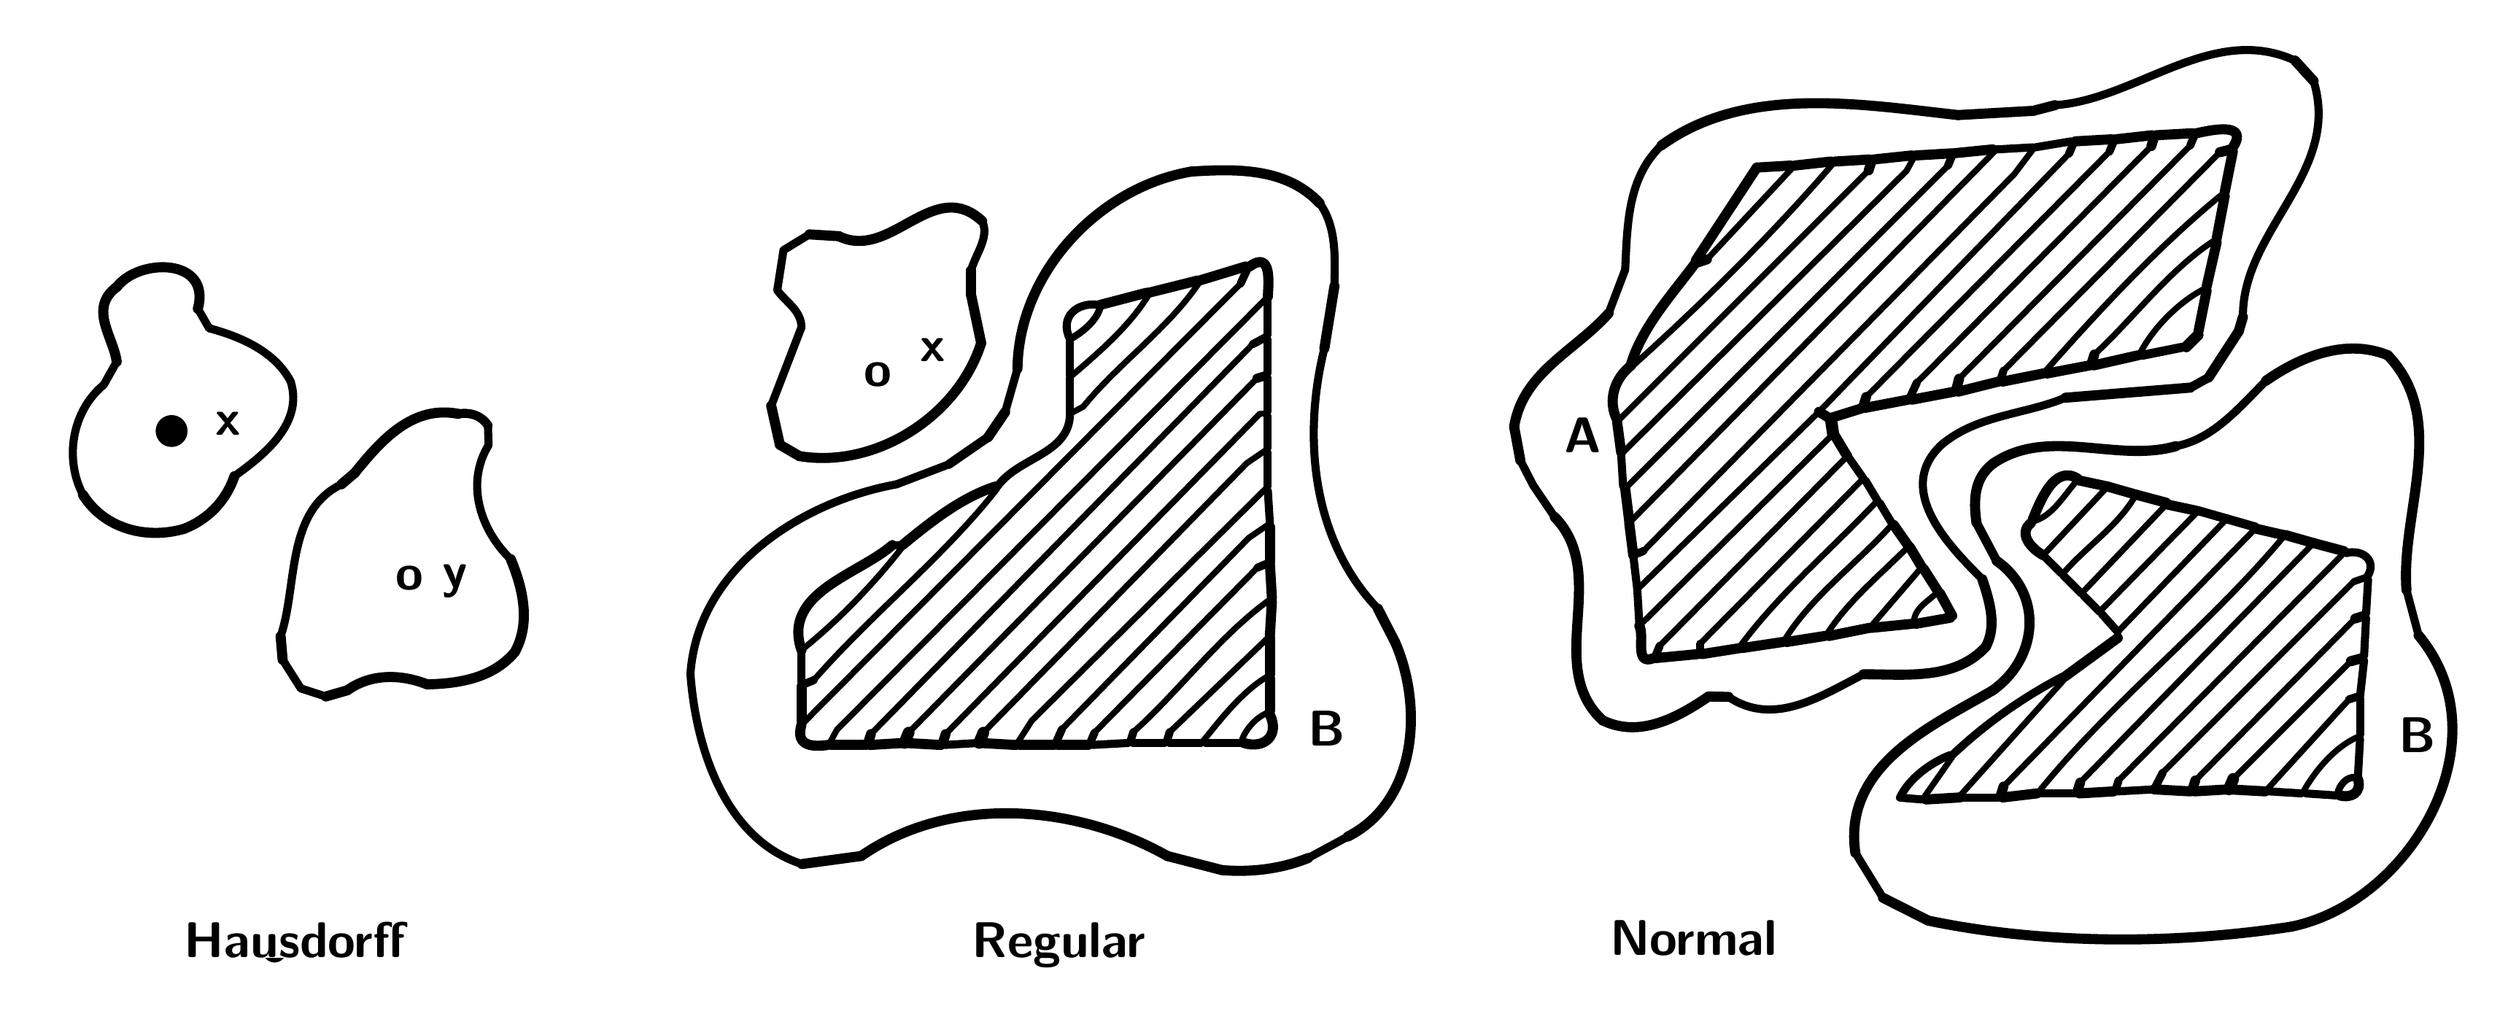
\begin{tikzpicture}[x=1pt, y=-1pt, line width=5.0pt, line cap=round, line join=round]

  %% ════ 填充区（prims2 的 fills）════

  %% ════ 直线段（prims2 的 strokes）════
  \draw[line width=5.0pt] (833.0,314.0) -- (852.0,311.0);
  \draw[line width=5.0pt] (939.0,299.0) -- (956.0,296.0);
  \draw[line width=4.0pt] (617.0,157.0) -- (610.5,160.5);
  \draw[line width=3.0pt] (610.5,160.5) -- (421.4,353.6);
  \draw[line width=4.9pt] (421.4,353.6) -- (420.0,358.0);
  \draw[line width=5.0pt] (1088.0,108.0) -- (1092.0,87.0);
  \draw[line width=5.0pt] (387.0,347.0) -- (387.0,330.0);
  \draw[line width=3.0pt] (1106.0,253.0) -- (982.4,379.6);
  \draw[line width=4.9pt] (982.4,379.6) -- (981.0,384.0);
  \draw[line width=5.0pt] (1048.0,235.0) -- (1034.0,231.0);
  \draw[line width=5.0pt] (1048.0,235.0) -- (1063.0,239.0);
  \draw[line width=4.0pt] (1162.0,296.0) -- (1161.0,315.0);
  \draw[line width=4.5pt] (617.0,176.0) -- (612.6,177.4);
  \draw[line width=3.0pt] (612.6,177.4) -- (440.1,352.9);
  \draw[line width=5.8pt] (440.1,352.9) -- (438.0,358.0);
  \draw[line width=5.0pt] (1112.0,382.0) -- (1094.0,381.0);
  \draw[line width=4.0pt] (957.0,67.0) -- (954.9,72.1);
  \draw[line width=3.0pt] (954.9,72.1) -- (796.0,231.0);
  \draw[line width=5.0pt] (1136.0,259.0) -- (1122.0,255.0);
  \draw[line width=5.0pt] (1136.0,259.0) -- (1151.0,263.0);
  \draw[line width=3.0pt] (1136.0,259.0) -- (1020.4,377.6);
  \draw[line width=4.9pt] (1020.4,377.6) -- (1019.0,382.0);
  \draw[line width=3.0pt] (878.0,73.0) -- (835.5,118.5);
  \draw[line width=4.9pt] (835.5,118.5) -- (831.0,120.0);
  \draw[line width=3.0pt] (617.0,138.0) -- (404.6,351.4);
  \draw[line width=3.0pt] (404.6,351.4) -- (401.0,358.0);
  \draw[line width=3.0pt] (1003.0,264.0) -- (1034.0,231.0);
  \draw[line width=5.0pt] (1002.0,175.0) -- (982.0,179.0);
  \draw[line width=5.0pt] (982.0,385.0) -- (999.0,383.0);
  \draw[line width=5.0pt] (875.0,308.0) -- (894.0,305.0);
  \draw[line width=3.0pt] (494.0,358.0) -- (501.1,346.9);
  \draw[line width=3.0pt] (501.1,346.9) -- (617.0,232.0);
  \draw[line width=4.0pt] (913.0,227.0) -- (906.0,217.0);
  \draw[line width=4.0pt] (794.0,231.0) -- (793.0,215.0);
  \draw[line width=5.0pt] (1027.0,171.0) -- (1049.0,166.0);
  \draw[line width=4.0pt] (914.0,228.0) -- (920.0,238.0);
  \draw[line width=4.0pt] (942.0,386.0) -- (931.1,385.1);
  \draw[line width=3.0pt] (803.0,299.0) -- (897.0,206.0);
  \draw[line width=4.0pt] (393.1,326.9) -- (388.0,329.0);
  \draw[line width=5.0pt] (1075.0,382.0) -- (1057.0,381.0);
  \draw[line width=4.5pt] (1051.0,166.0) -- (1071.0,162.0);
  \draw[line width=4.0pt] (832.0,313.0) -- (832.0,309.0);
  \draw[line width=3.0pt] (832.0,309.0) -- (912.0,228.0);
  \draw[line width=5.0pt] (619.0,251.0) -- (619.0,268.0);
  \draw[line width=4.0pt] (1011.0,274.0) -- (1003.0,266.0);
  \draw[line width=3.0pt] (1078.0,155.0) -- (1072.0,161.0);
  \draw[line width=5.0pt] (943.0,272.0) -- (950.0,283.0);
  \draw[line width=4.9pt] (457.0,358.0) -- (458.4,353.6);
  \draw[line width=3.0pt] (458.4,353.6) -- (614.0,195.0);
  \draw[line width=3.0pt] (614.0,195.0) -- (617.0,195.0);
  \draw[line width=5.0pt] (980.0,179.0) -- (960.0,184.0);
  \draw[line width=5.8pt] (475.0,358.0) -- (477.1,352.9);
  \draw[line width=3.0pt] (477.1,352.9) -- (607.6,219.4);
  \draw[line width=3.0pt] (607.6,219.4) -- (617.0,213.0);
  \draw[line width=4.0pt] (475.0,358.0) -- (458.0,359.0);
  \draw[line width=5.0pt] (475.0,358.0) -- (493.0,359.0);
  \draw[line width=6.0pt] (898.0,205.0) -- (897.0,198.0);
  \draw[line width=5.0pt] (529.0,359.0) -- (514.0,359.0);
  \draw[line width=5.0pt] (797.0,249.0) -- (799.0,265.0);
  \draw[line width=3.0pt] (1150.0,265.0) -- (1039.4,376.6);
  \draw[line width=4.0pt] (1039.4,376.6) -- (1038.0,381.0);
  \draw[line width=4.0pt] (1037.0,60.0) -- (1034.9,65.1);
  \draw[line width=3.0pt] (1034.9,65.1) -- (914.4,186.6);
  \draw[line width=4.9pt] (914.4,186.6) -- (913.0,191.0);
  \draw[line width=4.0pt] (569.0,358.0) -- (585.0,358.0);
  \draw[line width=4.0pt] (587.0,358.0) -- (604.0,358.0);
  \draw[line width=5.0pt] (937.0,299.0) -- (917.0,301.0);
  \draw[line width=5.0pt] (421.0,359.0) -- (438.0,358.0);
  \draw[line width=4.0pt] (927.0,249.0) -- (921.0,239.0);
  \draw[line width=5.0pt] (935.0,188.0) -- (914.0,192.0);
  \draw[line width=4.0pt] (520.0,177.0) -- (520.0,195.0);
  \draw[line width=4.0pt] (802.0,299.0) -- (801.0,282.0);
  \draw[line width=5.0pt] (1108.0,252.0) -- (1121.0,255.0);
  \draw[line width=4.0pt] (618.0,194.0) -- (618.0,177.0);
  \draw[line width=5.0pt] (937.0,67.0) -- (918.0,69.0);
  \draw[line width=3.0pt] (1062.0,241.0) -- (1022.0,283.0);
  \draw[line width=5.0pt] (607.0,122.0) -- (584.0,129.0);
  \draw[line width=5.0pt] (959.0,183.0) -- (960.4,177.6);
  \draw[line width=3.0pt] (960.4,177.6) -- (1074.9,62.1);
  \draw[line width=4.0pt] (1074.9,62.1) -- (1077.0,57.0);
  \draw[line width=3.0pt] (526.6,191.4) -- (520.0,195.0);
  \draw[line width=3.0pt] (388.0,348.0) -- (604.5,130.5);
  \draw[line width=4.0pt] (604.5,130.5) -- (608.0,123.0);
  \draw[line width=5.0pt] (1020.0,383.0) -- (1037.0,382.0);
  \draw[line width=5.0pt] (1036.0,59.0) -- (1018.0,60.0);
  \draw[line width=5.0pt] (438.0,358.0) -- (456.0,359.0);
  \draw[line width=5.0pt] (830.0,119.0) -- (860.2,73.0);
  \draw[line width=5.0pt] (860.2,73.0) -- (877.0,72.0);
  \draw[line width=4.0pt] (520.0,158.0) -- (520.0,176.0);
  \draw[line width=5.0pt] (873.0,308.0) -- (853.0,311.0);
  \draw[line width=4.0pt] (1132.0,383.0) -- (1147.0,384.0);
  \draw[line width=3.0pt] (997.0,64.0) -- (987.8,76.2);
  \draw[line width=3.0pt] (987.8,76.2) -- (804.1,262.9);
  \draw[line width=4.0pt] (804.1,262.9) -- (799.0,265.0);
  \draw[line width=4.5pt] (1107.0,251.0) -- (1093.0,247.0);
  \draw[line width=5.0pt] (402.0,359.0) -- (419.0,359.0);
  \draw[line width=4.0pt] (618.0,139.0) -- (618.0,156.0);
  \draw[line width=5.0pt] (935.0,260.0) -- (928.0,250.0);
  \draw[line width=3.0pt] (957.0,365.0) -- (943.0,385.0);
  \draw[line width=4.0pt] (1159.0,336.0) -- (1159.0,354.0);
  \draw[line width=4.0pt] (618.0,196.0) -- (618.0,212.0);
  \draw[line width=5.0pt] (913.0,192.0) -- (897.0,197.0);
  \draw[line width=4.0pt] (618.0,158.0) -- (618.0,175.0);
  \draw[line width=4.5pt] (1079.0,243.0) -- (1093.0,247.0);
  \draw[line width=5.0pt] (619.0,306.0) -- (619.0,324.0);
  \draw[line width=4.9pt] (1076.0,381.0) -- (1077.4,376.6);
  \draw[line width=3.0pt] (1077.4,376.6) -- (1156.6,296.4);
  \draw[line width=4.9pt] (1156.6,296.4) -- (1161.0,295.0);
  \draw[line width=5.0pt] (1096.0,65.0) -- (1092.0,85.0);
  \draw[line width=4.9pt] (1057.0,58.0) -- (1055.6,62.4);
  \draw[line width=3.0pt] (1055.6,62.4) -- (939.5,179.5);
  \draw[line width=4.0pt] (939.5,179.5) -- (936.0,187.0);
  \draw[line width=4.0pt] (1159.0,356.0) -- (1158.0,374.0);
  \draw[line width=4.0pt] (801.0,282.0) -- (799.0,265.0);
  \draw[line width=3.0pt] (801.0,282.0) -- (891.0,194.0);
  \draw[line width=4.0pt] (549.0,358.0) -- (531.0,359.0);
  \draw[line width=5.0pt] (1079.0,156.0) -- (1073.0,162.0);
  \draw[line width=4.0pt] (1031.0,294.0) -- (1039.0,303.0);
  \draw[line width=4.0pt] (567.0,358.0) -- (551.0,358.0);
  \draw[line width=3.0pt] (961.0,384.0) -- (1013.0,326.0);
  \draw[line width=4.0pt] (551.4,352.6) -- (550.0,357.0);
  \draw[line width=3.0pt] (798.0,248.0) -- (978.0,65.0);
  \draw[line width=5.0pt] (495.0,359.0) -- (512.0,359.0);
  \draw[line width=4.0pt] (619.0,249.0) -- (618.0,233.0);
  \draw[line width=5.0pt] (795.0,232.0) -- (797.0,248.0);
  \draw[line width=5.0pt] (1064.0,240.0) -- (1078.0,243.0);
  \draw[line width=3.0pt] (618.0,306.0) -- (569.4,352.6);
  \draw[line width=4.0pt] (569.4,352.6) -- (568.0,357.0);
  \draw[line width=4.0pt] (1057.0,381.0) -- (1061.3,372.7);
  \draw[line width=3.0pt] (1061.3,372.7) -- (1155.9,278.1);
  \draw[line width=3.5pt] (1155.9,278.1) -- (1162.0,276.0);
  \draw[line width=4.0pt] (1057.0,381.0) -- (1039.0,382.0);
  \draw[line width=4.0pt] (432.0,260.0) -- (436.0,260.0);
  \draw[line width=4.0pt] (387.0,312.0) -- (387.0,328.0);
  \draw[line width=3.0pt] (792.0,198.0) -- (915.6,74.4);
  \draw[line width=4.9pt] (915.6,74.4) -- (917.0,70.0);
  \draw[line width=4.0pt] (981.0,178.0) -- (982.4,173.6);
  \draw[line width=3.0pt] (982.4,173.6) -- (1089.6,65.4);
  \draw[line width=5.0pt] (1089.6,65.4) -- (1095.0,64.0);
  \draw[line width=5.0pt] (899.0,70.0) -- (916.0,69.0);
  \draw[line width=4.0pt] (530.0,358.0) -- (532.2,352.8);
  \draw[line width=3.0pt] (532.2,352.8) -- (612.8,271.2);
  \draw[line width=4.0pt] (612.8,271.2) -- (618.0,269.0);
  \draw[line width=5.0pt] (977.0,64.0) -- (957.0,66.0);
  \draw[line width=3.0pt] (938.0,68.0) -- (934.4,74.6);
  \draw[line width=3.0pt] (934.4,74.6) -- (794.0,214.0);
  \draw[line width=5.0pt] (899.0,206.0) -- (905.0,216.0);
  \draw[line width=5.0pt] (896.0,305.0) -- (916.0,301.0);
  \draw[line width=5.0pt] (1076.0,56.0) -- (1058.0,57.0);
  \draw[line width=3.0pt] (904.0,217.0) -- (812.1,309.9);
  \draw[line width=4.0pt] (812.1,309.9) -- (810.0,315.0);
  \draw[line width=5.0pt] (1088.0,110.0) -- (1083.0,132.0);
  \draw[line width=5.0pt] (1013.0,325.0) -- (1039.0,306.0);
  \draw[line width=4.0pt] (1012.0,275.0) -- (1021.0,284.0);
  \draw[line width=5.0pt] (831.0,314.0) -- (810.0,316.0);
  \draw[line width=4.9pt] (1027.4,165.6) -- (1026.0,170.0);
  \draw[line width=5.0pt] (957.0,295.0) -- (951.0,284.0);
  \draw[line width=5.0pt] (559.0,135.0) -- (583.0,129.0);
  \draw[line width=4.0pt] (962.0,385.0) -- (980.0,385.0);
  \draw[line width=5.0pt] (620.0,286.0) -- (619.0,269.0);
  \draw[line width=3.0pt] (1113.0,381.0) -- (1153.6,336.4);
  \draw[line width=4.0pt] (1153.6,336.4) -- (1158.0,335.0);
  \draw[line width=5.0pt] (1020.0,228.0) -- (1034.0,231.0);
  \draw[line width=4.0pt] (618.0,214.0) -- (618.0,231.0);
  \draw[line width=5.0pt] (1160.0,316.0) -- (1154.5,317.5);
  \draw[line width=3.0pt] (1154.5,317.5) -- (1096.2,375.8);
  \draw[line width=5.8pt] (1096.2,375.8) -- (1094.0,381.0);
  \draw[line width=4.0pt] (1114.0,382.0) -- (1130.0,383.0);
  \draw[line width=5.0pt] (1025.0,171.0) -- (1004.0,175.0);
  \draw[line width=5.0pt] (936.0,261.0) -- (942.0,271.0);
  \draw[line width=5.0pt] (558.0,135.0) -- (535.0,141.0);
  \draw[line width=5.0pt] (619.0,342.0) -- (619.0,326.0);
  \draw[line width=4.0pt] (1159.0,335.0) -- (1161.0,317.0);
  \draw[line width=3.0pt] (891.0,194.0) -- (1014.9,66.1);
  \draw[line width=4.0pt] (1014.9,66.1) -- (1017.0,61.0);
  \draw[line width=5.0pt] (891.0,194.0) -- (896.0,197.0);
  \draw[line width=4.0pt] (1163.0,277.0) -- (1162.0,294.0);
  \draw[line width=5.0pt] (620.0,288.0) -- (619.0,305.0);
  \draw[line width=5.0pt] (879.0,72.0) -- (897.0,70.0);
  \draw[line width=3.0pt] (941.0,272.0) -- (917.0,300.0);
  \draw[line width=5.0pt] (961.0,385.0) -- (944.0,386.0);
  \draw[line width=5.0pt] (1094.0,381.0) -- (1077.0,382.0);
  \draw[line width=5.0pt] (1083.0,134.0) -- (1079.0,154.0);
  \draw[line width=3.0pt] (1031.0,292.0) -- (1078.0,244.0);
  \draw[line width=5.0pt] (958.0,184.0) -- (937.0,188.0);
  \draw[line width=11.5pt] (130.0,454.0) -- (126.0,461.0);
  \draw[line width=4.0pt] (1000.0,383.0) -- (1018.0,383.0);
  \draw[line width=4.0pt] (1022.0,285.0) -- (1030.0,293.0);
  \draw[line width=4.0pt] (1016.0,60.0) -- (998.0,63.0);
  \draw[line width=5.0pt] (956.0,66.0) -- (939.0,67.0);
  \draw[line width=3.0pt] (1039.0,303.0) -- (1093.0,247.0);
  \draw[line width=5.0pt] (1038.0,59.0) -- (1056.0,57.0);
  \draw[line width=3.0pt] (618.0,250.0) -- (608.6,256.4);
  \draw[line width=3.0pt] (608.6,256.4) -- (516.0,351.2);
  \draw[line width=4.0pt] (516.0,351.2) -- (513.0,358.0);
  \draw[line width=5.0pt] (791.0,199.0) -- (793.0,214.0);
  \draw[line width=4.0pt] (997.0,63.0) -- (979.0,64.0);
  \draw[line width=4.0pt] (638.0,415.0) -- (657.6,404.4);
  \draw[line width=5.0pt] (681.0,308.0) -- (672.5,291.5);
  \draw[line width=5.0pt] (646.0,162.6) -- (651.0,131.7);
  \draw[line width=4.0pt] (494.0,172.6) -- (487.9,194.1);
  \draw[line width=5.0pt] (487.9,194.1) -- (479.4,206.6);
  \draw[line width=4.5pt] (479.4,206.6) -- (460.0,220.0);
  \draw[line width=4.0pt] (460.0,220.0) -- (434.1,229.9);
  \draw[line width=5.0pt] (387.2,418.0) -- (416.6,414.0);
  \draw[line width=5.0pt] (568.2,414.0) -- (595.3,421.0);
  \draw[line width=5.0pt] (1084.0,177.0) -- (1098.9,154.1);
  \draw[line width=5.0pt] (1098.9,154.1) -- (1101.0,147.0);
  \draw[line width=5.0pt] (1136.0,30.1) -- (1126.8,20.0);
  \draw[line width=5.0pt] (1007.9,42.1) -- (997.1,44.9);
  \draw[line width=5.0pt] (997.1,44.9) -- (959.9,47.0);
  \draw[line width=4.0pt] (795.0,123.6) -- (786.8,145.2);
  \draw[line width=5.0pt] (740.0,201.4) -- (743.1,218.1);
  \draw[line width=4.0pt] (743.1,218.1) -- (749.5,230.5);
  \draw[line width=4.0pt] (749.5,230.5) -- (760.1,246.1);
  \draw[line width=5.0pt] (836.3,335.0) -- (846.2,335.2);
  \draw[line width=5.0pt] (1013.1,187.0) -- (1075.0,182.0);
  \draw[line width=4.5pt] (1075.0,182.0) -- (1084.0,177.0);
  \draw[line width=4.0pt] (372.0,191.0) -- (387.0,152.1);
  \draw[line width=4.0pt] (375.0,133.7) -- (378.1,113.9);
  \draw[line width=4.0pt] (378.1,113.9) -- (390.9,106.1);
  \draw[line width=5.0pt] (390.9,106.1) -- (405.5,107.0);
  \draw[line width=5.0pt] (471.0,124.0) -- (471.0,136.0);
  \draw[line width=5.0pt] (471.0,136.0) -- (476.0,159.9);
  \draw[line width=5.0pt] (385.9,215.9) -- (376.3,210.3);
  \draw[line width=5.0pt] (376.3,210.3) -- (372.0,191.0);
  \draw[line width=5.0pt] (945.1,446.0) -- (922.7,434.7);
  \draw[line width=4.0pt] (922.7,434.7) -- (909.0,412.4);
  \draw[line width=4.5pt] (979.0,267.8) -- (969.0,248.9);
  \draw[line width=4.0pt] (1182.0,282.2) -- (1188.0,304.7);
  \draw[line width=4.0pt] (88.0,142.9) -- (93.6,152.6);
  \draw[line width=4.0pt] (41.4,180.6) -- (47.8,169.2);
  \draw[line width=5.0pt] (165.7,224.3) -- (159.1,229.9);
  \draw[line width=5.0pt] (129.0,305.2) -- (130.0,316.8);
  \draw[line width=4.0pt] (130.0,316.8) -- (139.0,331.0);
  \draw[line width=4.0pt] (139.0,331.0) -- (151.4,335.0);
  \draw[line width=5.0pt] (151.4,335.0) -- (162.1,331.9);
  \draw[line width=4.0pt] (232.0,210.5) -- (231.7,200.7);

  %% ════ 曲线（prims2 的 curves —— 三段式，坐标同为 (y,x)）════
  \draw[line width=5.0pt] (798.0,170.0) .. controls (803.9,151.3) and (818.2,135.9) .. (830.0,120.0);
  \draw[line width=3.0pt] (799.0,171.0) .. controls (832.8,140.7) and (868.1,105.8) .. (898.0,71.0);
  \draw[line width=3.0pt] (1000.0,382.0) .. controls (1036.5,337.0) and (1084.2,300.0) .. (1121.0,256.0);
  \draw[line width=3.0pt] (1048.0,235.0) .. controls (1039.8,250.1) and (1023.0,261.0) .. (1012.0,274.0);
  \draw[line width=3.0pt] (618.0,343.0) .. controls (612.3,345.2) and (606.9,351.2) .. (605.0,357.0);
  \draw[line width=5.0pt] (1149.0,384.0) .. controls (1154.8,385.5) and (1159.9,382.5) .. (1158.0,376.0);
  \draw[line width=3.0pt] (919.0,239.0) .. controls (896.6,262.6) and (870.8,284.5) .. (852.0,310.0);
  \draw[line width=3.0pt] (1091.0,86.0) .. controls (1059.7,111.4) and (1029.6,143.9) .. (1003.0,174.0);
  \draw[line width=5.0pt] (606.0,358.0) .. controls (616.5,361.2) and (623.9,354.1) .. (619.0,344.0);
  \draw[line width=4.0pt] (931.1,385.1) .. controls (935.5,375.7) and (946.4,367.7) .. (956.0,364.0);
  \draw[line width=3.0pt] (484.0,232.0) .. controls (458.0,265.3) and (421.7,294.2) .. (393.1,326.9);
  \draw[line width=3.0pt] (895.0,304.0) .. controls (905.4,287.7) and (921.5,274.6) .. (935.0,261.0);
  \draw[line width=3.0pt] (584.0,130.0) .. controls (568.8,152.6) and (543.7,170.3) .. (526.6,191.4);
  \draw[line width=5.0pt] (1019.0,227.0) .. controls (1007.4,219.9) and (1000.3,239.1) .. (997.0,247.0);
  \draw[line width=4.0pt] (520.0,158.0) .. controls (514.6,147.2) and (523.3,139.5) .. (534.0,141.0);
  \draw[line width=3.5pt] (520.0,158.0) .. controls (525.9,154.8) and (533.4,148.8) .. (535.0,142.0);
  \draw[line width=4.0pt] (1152.0,264.0) .. controls (1159.7,261.9) and (1167.3,267.1) .. (1163.0,275.0);
  \draw[line width=3.0pt] (619.0,287.0) .. controls (594.3,304.7) and (574.4,332.0) .. (551.4,352.6);
  \draw[line width=3.0pt] (1082.0,133.0) .. controls (1069.3,139.5) and (1056.7,152.2) .. (1050.0,165.0);
  \draw[line width=3.0pt] (1158.0,355.0) .. controls (1146.9,359.7) and (1136.8,371.6) .. (1131.0,382.0);
  \draw[line width=3.0pt] (1018.0,229.0) .. controls (1012.3,235.6) and (1006.8,245.1) .. (998.0,248.0);
  \draw[line width=5.0pt] (996.0,249.0) .. controls (989.4,254.5) and (996.4,261.9) .. (1002.0,265.0);
  \draw[line width=5.0pt] (387.0,312.0) .. controls (377.3,283.5) and (415.2,274.7) .. (432.0,260.0);
  \draw[line width=3.0pt] (387.0,312.0) .. controls (405.1,297.6) and (422.9,279.1) .. (437.0,261.0);
  \draw[line width=3.0pt] (618.0,325.0) .. controls (605.8,332.0) and (594.9,345.9) .. (586.0,357.0);
  \draw[line width=5.0pt] (798.0,171.0) .. controls (789.6,177.5) and (786.2,188.4) .. (791.0,198.0);
  \draw[line width=3.0pt] (949.0,284.0) .. controls (944.7,288.0) and (938.3,291.5) .. (938.0,298.0);
  \draw[line width=3.0pt] (1087.0,109.0) .. controls (1064.4,123.6) and (1047.7,146.8) .. (1027.4,165.6);
  \draw[line width=5.0pt] (437.0,260.0) .. controls (451.1,248.4) and (466.1,236.5) .. (483.0,231.0);
  \draw[line width=3.0pt] (927.0,250.0) .. controls (909.8,269.1) and (886.8,285.9) .. (874.0,307.0);
  \draw[line width=5.0pt] (1096.0,63.0) .. controls (1104.4,50.1) and (1084.7,54.5) .. (1078.0,56.0);
  \draw[line width=5.0pt] (618.0,137.0) .. controls (618.3,129.9) and (620.1,114.0) .. (609.0,122.0);
  \draw[line width=5.0pt] (387.0,349.0) .. controls (383.9,359.2) and (391.8,360.2) .. (400.0,359.0);
  \draw[line width=3.5pt] (1148.0,383.0) .. controls (1148.9,378.7) and (1152.2,374.7) .. (1157.0,375.0);
  \draw[line width=4.0pt] (484.0,231.0) .. controls (494.4,216.4) and (519.8,215.0) .. (520.0,195.0);
  \draw[line width=3.0pt] (521.0,176.0) .. controls (534.4,164.5) and (549.7,151.3) .. (559.0,136.0);
  \draw[line width=4.0pt] (1012.0,325.0) .. controls (992.3,335.2) and (973.7,348.3) .. (957.0,364.0);
  \draw[line width=5.0pt] (802.0,300.0) .. controls (804.8,304.8) and (799.3,319.9) .. (809.0,316.0);
  \draw[line width=5.0pt] (657.6,404.4) .. controls (692.1,386.8) and (695.0,339.8) .. (681.0,308.0);
  \draw[line width=4.0pt] (672.5,291.5) .. controls (640.1,257.7) and (635.0,207.0) .. (646.0,162.6);
  \draw[line width=4.0pt] (651.0,131.7) .. controls (651.2,117.2) and (652.1,102.5) .. (643.7,90.7);
  \draw[line width=5.0pt] (643.7,90.7) .. controls (627.4,73.1) and (602.3,73.5) .. (580.0,75.0);
  \draw[line width=5.0pt] (580.0,75.0) .. controls (534.2,82.8) and (494.5,125.2) .. (494.0,172.6);
  \draw[line width=4.0pt] (434.1,229.9) .. controls (387.2,238.4) and (335.6,271.2) .. (332.0,323.8);
  \draw[line width=4.0pt] (332.0,323.8) .. controls (334.6,360.1) and (348.9,405.6) .. (387.2,418.0);
  \draw[line width=5.0pt] (416.6,414.0) .. controls (461.1,383.2) and (523.0,388.5) .. (568.2,414.0);
  \draw[line width=5.0pt] (595.3,421.0) .. controls (610.0,422.2) and (624.6,420.4) .. (638.0,415.0);
  \draw[line width=4.0pt] (1101.0,147.0) .. controls (1100.5,104.0) and (1150.0,75.5) .. (1136.0,30.1);
  \draw[line width=4.0pt] (1126.8,20.0) .. controls (1085.7,1.1) and (1048.3,39.4) .. (1007.9,42.1);
  \draw[line width=5.0pt] (959.9,47.0) .. controls (911.3,41.6) and (854.6,31.9) .. (813.0,62.0);
  \draw[line width=4.0pt] (813.0,62.0) .. controls (796.0,78.1) and (796.1,101.7) .. (795.0,123.6);
  \draw[line width=5.0pt] (786.8,145.2) .. controls (770.2,163.9) and (744.3,174.3) .. (740.0,201.4);
  \draw[line width=5.0pt] (760.1,246.1) .. controls (787.8,274.7) and (754.7,319.9) .. (783.8,346.8);
  \draw[line width=5.0pt] (783.8,346.8) .. controls (802.3,355.8) and (821.2,345.3) .. (836.3,335.0);
  \draw[line width=4.0pt] (846.2,335.2) .. controls (868.8,350.4) and (892.6,334.4) .. (913.0,324.0);
  \draw[line width=5.0pt] (913.0,324.0) .. controls (933.8,323.9) and (958.1,327.2) .. (973.6,310.4);
  \draw[line width=5.0pt] (973.6,310.4) .. controls (979.3,300.0) and (975.4,287.5) .. (971.9,276.9);
  \draw[line width=4.0pt] (971.9,276.9) .. controls (954.9,260.0) and (928.2,232.3) .. (951.7,210.3);
  \draw[line width=4.0pt] (951.7,210.3) .. controls (969.4,195.4) and (992.9,195.4) .. (1013.1,187.0);
  \draw[line width=4.0pt] (387.0,152.1) .. controls (386.8,143.6) and (379.4,139.9) .. (375.0,133.7);
  \draw[line width=5.0pt] (405.5,107.0) .. controls (431.2,119.5) and (452.3,77.0) .. (476.5,99.5);
  \draw[line width=4.0pt] (476.5,99.5) .. controls (480.3,107.6) and (473.1,116.0) .. (471.0,124.0);
  \draw[line width=5.0pt] (476.0,159.9) .. controls (464.7,195.9) and (423.9,222.3) .. (385.9,215.9);
  \draw[line width=5.0pt] (1125.0,449.0) .. controls (1067.1,457.9) and (1001.9,457.9) .. (945.1,446.0);
  \draw[line width=5.0pt] (909.0,412.4) .. controls (902.8,368.9) and (946.8,349.6) .. (977.0,332.0);
  \draw[line width=5.0pt] (977.0,332.0) .. controls (999.7,315.9) and (1002.3,284.3) .. (979.0,267.8);
  \draw[line width=5.0pt] (969.0,248.9) .. controls (967.5,237.8) and (967.6,226.6) .. (977.7,219.3);
  \draw[line width=5.0pt] (977.7,219.3) .. controls (1004.8,201.3) and (1038.7,219.4) .. (1067.8,211.0);
  \draw[line width=4.0pt] (1067.8,211.0) .. controls (1086.2,207.5) and (1099.1,192.0) .. (1112.4,178.6);
  \draw[line width=5.0pt] (1112.4,178.6) .. controls (1129.4,166.7) and (1152.0,157.4) .. (1172.8,166.0);
  \draw[line width=5.0pt] (1172.8,166.0) .. controls (1203.2,197.9) and (1179.1,243.5) .. (1182.0,282.2);
  \draw[line width=5.0pt] (1188.0,304.7) .. controls (1231.0,356.4) and (1184.4,436.8) .. (1125.0,449.0);
  \draw[line width=5.0pt] (48.0,132.0) .. controls (58.9,117.8) and (94.8,117.6) .. (88.0,142.9);
  \draw[line width=4.0pt] (93.6,152.6) .. controls (108.9,156.7) and (126.1,163.9) .. (134.0,179.0);
  \draw[line width=4.0pt] (134.0,179.0) .. controls (140.4,199.7) and (121.0,215.2) .. (106.1,225.9);
  \draw[line width=5.0pt] (106.1,225.9) .. controls (102.1,237.8) and (93.2,247.3) .. (81.0,252.0);
  \draw[line width=5.0pt] (81.0,252.0) .. controls (62.7,257.2) and (41.9,252.2) .. (31.1,235.1);
  \draw[line width=4.0pt] (31.1,235.1) .. controls (21.8,217.4) and (25.5,193.7) .. (41.4,180.6);
  \draw[line width=5.0pt] (47.8,169.2) .. controls (46.3,156.9) and (33.5,142.7) .. (48.0,132.0);
  \draw[line width=5.0pt] (217.0,195.0) .. controls (194.4,190.6) and (179.0,207.8) .. (165.7,224.3);
  \draw[line width=4.0pt] (159.1,229.9) .. controls (131.4,243.5) and (137.5,280.2) .. (129.0,305.2);
  \draw[line width=5.0pt] (162.1,331.9) .. controls (173.8,323.5) and (188.8,323.9) .. (201.6,329.0);
  \draw[line width=5.0pt] (201.6,329.0) .. controls (217.6,328.6) and (234.1,325.9) .. (245.0,313.0);
  \draw[line width=5.0pt] (245.0,313.0) .. controls (253.0,298.6) and (249.0,281.3) .. (243.0,267.0);
  \draw[line width=4.0pt] (243.0,267.0) .. controls (227.8,252.4) and (220.5,229.3) .. (232.0,210.5);
  \draw[line width=4.5pt] (231.7,200.7) .. controls (228.2,195.6) and (222.9,194.1) .. (217.0,195.0);

  %% ════ 实心点 ════
  \fill (75.0,203.5) circle (7.9);

  %% ════ 标签（probe 直接给的 \node 行）════
  %% ⚠ 全部补了 fill=white：文字在最上层，否则与曲线交叉干扰
     \node[anchor=center,inner sep=0pt,fill=white,font=\fontsize{29.2}{36.5}\selectfont] at (452.0,163.4) {\textsf{\textbf{\textit{x}}}};   % box(443,153,16,17)
     \node[anchor=center,inner sep=0pt,fill=white,font=\fontsize{29.5}{36.9}\selectfont] at (424.7,175.5) {\textsf{\textbf{\textit{o}}}};   % box(416,166,16,16)
     \node[anchor=center,inner sep=0pt,fill=white,font=\fontsize{28.3}{35.4}\selectfont] at (102.9,199.9) {\textsf{\textbf{\textit{x}}}};   % box(94,190,16,16)
     \node[anchor=center,inner sep=0pt,fill=white,font=\fontsize{29.6}{37.0}\selectfont] at (774.2,205.5) {\textsf{\textbf{\textit{A}}}};   % box(762,194,19,22)
     \node[anchor=center,inner sep=0pt,fill=white,font=\fontsize{29.2}{36.4}\selectfont] at (215.7,277.7) {\textsf{\textbf{\textit{y}}}};   % box(207,265,17,22)
     \node[anchor=center,inner sep=0pt,fill=white,font=\fontsize{29.5}{36.9}\selectfont] at (192.7,276.5) {\textsf{\textbf{\textit{o}}}};   % box(184,267,16,16)
     \node[anchor=center,inner sep=0pt,fill=white,font=\fontsize{30.2}{37.8}\selectfont] at (647.3,351.0) {\textsf{\textbf{\textit{B}}}};   % box(636,339,19,23)
     \node[anchor=center,inner sep=0pt,fill=white,font=\fontsize{30.2}{37.8}\selectfont] at (1187.3,354.0) {\textsf{\textbf{\textit{B}}}};   % box(1176,342,19,23)
     \node[anchor=center,inner sep=0pt,fill=white,font=\fontsize{29.7}{37.1}\selectfont] at (514.7,458.2) {\textsf{\textbf{\textit{Regular}}}};   % box(460,443,106,29)
     \node[anchor=center,inner sep=0pt,fill=white,font=\fontsize{29.3}{36.7}\selectfont] at (829.0,454.7) {\textsf{\textbf{\textit{Normal}}}};   % box(779,443,98,22)
     \node[anchor=center,inner sep=0pt,fill=white,font=\fontsize{29.0}{36.2}\selectfont] at (137.0,455.7) {\textsf{\textbf{\textit{Hausdorff}}}};   % box(70,444,134,22)

  % 钉死画布：否则超出的图元/控制点会把页面撑大，1:1 回比就失准
  \pgfresetboundingbox
  \path[use as bounding box] (0,0) rectangle (1218,482);
\end{tikzpicture}
\end{document}

% ⚠ 待核清单（probe 拿不准，人眼过一遍）：
%   · 可疑字形：\node[anchor=center,inner sep=0pt,font=\fontsize{29.5}{36.9}\selectfont] at (424.7,175.5) {\textsf{\textbf{\te
%   · 可疑字形：\node[anchor=center,inner sep=0pt,font=\fontsize{29.5}{36.9}\selectfont] at (192.7,276.5) {\textsf{\textbf{\te
%   · 未识别/跳过：⑤ 跳过/未识别的字形
